%==============================
\section{Collaborative Optimal Transport under Signal Temporal Logic Tasks}
\label{ch06:sec:ch06_stl}


Multi-robot systems have been deployed in practice for numerous tasks,
such as service, maintenance, and search and rescue.
As a fundamental requirement, the system should be able to
navigate safely within a given complex workspace~\cite{lavalle2006planning},
i.e., to drive the robots from an initial state to the target state
while staying within the allowed workspace and avoiding
collision with obstacles or other robots.
In addition, the system is often subject to various constraints and high-level tasks,
e.g., the dynamics can be nonlinear;
to follow a relative formation~\cite{olfati2007consensus, guo2016communication,herguedas2022multi};
to remain connected during motion for information
exchange~\cite{sabattini2013distributed,antonelli2014decentralized};
and to fulfill task specifications in temporal logics~\cite{chen2021decentralized,lindemann2025formal}.
Addressing such objectives and constraints simultaneously can be challenging
due to their non-convexity and often conflicting goals.


This work addresses multi-robot planning from a novel perspective,
formulating it as a collaborative trajectory optimization task.
From a planning-as-inference view, trajectories are sampled from
Gaussian Process priors for smoothness, while dynamics and task
constraints are incorporated as costs.
A gradient-free method termed collaborative optimal transport (CLOT) is introduced,
which optimizes batches of smooth trajectories under highly nonlinear costs.
The Sinkhorn Step provides fast, zero-order, and parallelizable updates
that collaboratively transport trajectory waypoints toward low-cost regions.
To improve scalability, the scheme is extended with search over robot planning
sequences and coupled local optimizations.
The framework is applicable to complex workspaces with convex, non-convex,
or dynamic obstacles, and high-level signal temporal logic (STL) tasks.
Extensive numerical simulations and hardware experiments demonstrate its effectiveness.

Main contribution of this work is \emph{threefold}:
(I) it provides an alternative approach for multi-robot motion planning
under complex constraints and objectives, applicable to a wide range of scenarios;
(II) it demonstrates advantages compared to popular analytical planners
and sampling-based motion planners;
(III) it exemplifies the efficient usage of modern hardware such as GPUs
for multi-robot planning.


\subsection{Batch Computation of STL Perturbed Robustness}\label{ch06:subsec:batch-stl}
To enable batch optimization of trajectories, this section describes how to efficiently
evaluate the change in robustness when a single waypoint is perturbed in multiple directions.

%%===================
\subsubsection{Tree Structure of STL}\label{ch06:subsec:stl-tree}
An STL formula $\phi$ can be recursively decomposed into subformulas and operators
\cite{leung2023backpropagation}, which can be organized as a tree
\cite{kurtz2022mixed}. The STL tree is
$\mathcal{T}^{\phi}\triangleq (\widehat{\mathcal{T}}, \mathcal{I}, \circ)$,
where $\widehat{\mathcal{T}}=[\mathcal{T}^{\phi_{1}},\cdots,\mathcal{T}^{\phi_{K}}]$
is the list of $K\geq1$ subtrees, $\mathcal{I}=[I^{\phi_{1}},\cdots,I^{\phi_{K}}]$
are the time intervals, and $\circ\in\{\wedge,\vee\}$ are Boolean operators.
Temporal operators expand as: $\mathsf{F}_I$ to disjunction $\vee$,
$\mathsf{G}_I$ to conjunction $\wedge$, and $\mathsf{U}_I$ into a recursive
combination. Thus, $\mathcal{T}^\phi$ is recursive, leaves correspond to
predicates at time instants, and parent nodes represent operators.
An example is shown in Fig.~\ref{ch06:fig:stl-tree}.
%==============================
\begin{figure}[t!]
  \centering
  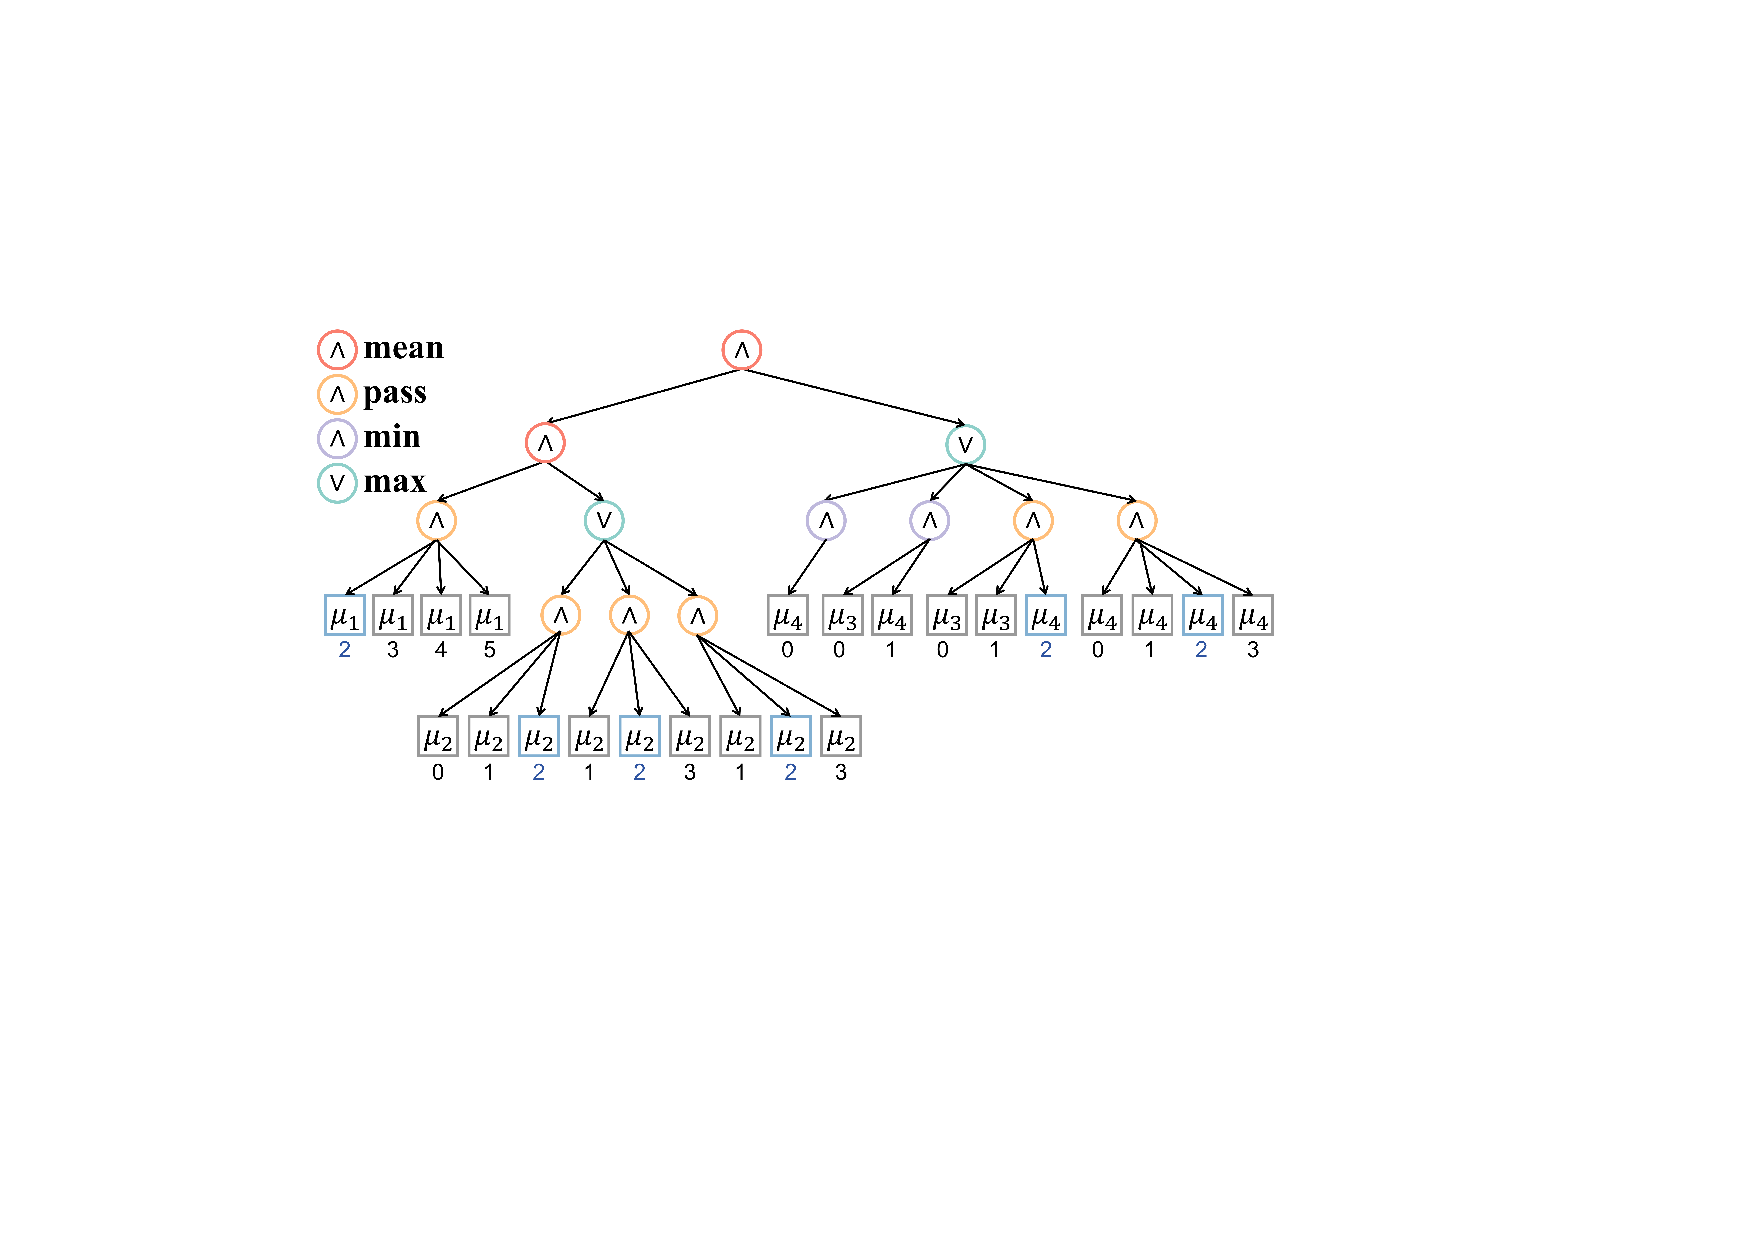
\includegraphics[width=0.95\hsize]{figures/ch06/stltree.pdf}
  \vspace{-0.1in}
  \caption{
    The STL tree and perturbed robustness evaluation
    for formula~$\phi = \big{(}\mathsf{G}_{[2,5]}\mu_1\big{)} \land
      \big{(}\mathsf{F}_{[0,2]}\mathsf{G}_{[0,2]}\mu_2\big{)}
      \land \big{(}\mu_3 \mathsf{U}_{[0,3]}\mu_4\big{)}$,
      with the $2$nd waypoint perturbed.
           }
  \label{ch06:fig:stl-tree}
  \vspace{-0.2in}
\end{figure}
% ==============================

%% ========================================
\subsubsection{Parallel Evaluation of Perturbed Robustness}\label{ch06:subsec:stl-robustness}
As in Sec.~\ref{ch06:subsec:robust}, robustness of a trajectory $\mathbf{Z}(T)$ is computed
recursively on $\mathcal{T}^{\phi}$ by evaluating leaves and applying
$\textbf{min}$ for conjunctions and $\textbf{max}$ for disjunctions
\cite{fainekos2009robustness,kurtz2022mixed,leung2023backpropagation}.
However, this may suppress perturbations, since a perturbed leaf dominated by
$\textbf{min}$ is discarded. To retain sensitivity, modified rules are used
when only the $t^\star$-th waypoint is perturbed, denoted
$\widehat{\mathbf{Z}}_{t^\star}(T)$: (I) leaf nodes
calculate pointwise robustness $f^k_i(\widehat{\mathbf{z}}(t))$;
(II) immediate conjunction parents pass
$f^k_i(\widehat{\mathbf{z}}(t^\star))$ upward if $t^\star\in I^{\phi_{i}}$;
(III) higher-level conjunctions aggregate via \textbf{mean}; and
(IV) disjunctions use standard \textbf{max}. The perturbed robustness is
\begin{equation*}\label{ch06:eq:perturbed-robustness}
  \widehat{\rho}^\phi\big(\widehat{\mathbf{Z}}_{t^\star}(T)\big) \triangleq
\texttt{Eval}_{\mathcal{T}^\phi} \Big(
  \{f^k_i(\widehat{\mathbf{z}}(t))\},
 \{\textbf{max},\textbf{min},\textbf{mean}\}\Big),
\end{equation*}
where $\texttt{Eval}_{\mathcal{T}^\phi}(\cdot)$ denotes the recursive evaluation with
modified operators. This amplifies the perturbation effects while approximating STL semantics,
enabling efficient batch evaluation across all perturbations for each robot.
% While $\widehat{\rho}^\phi$ guides optimization,
% final feasibility is strictly verified using standard STL semantics.


%==============================
\subsection{Sequential Local Optimal Transport}\label{ch06:sec:local}
Given the batch evaluation of STL robustness,
this section formalizes the sequential planning framework
based on local optimal transport.
The high-dimensional multi-robot planning problem
is decomposed into a sequence of lower-dimensional subproblems,
each optimizing one robot's trajectory in a prescribed order,
with previously planned trajectories incorporated as dynamic constraints.
% are treated as dynamic constraints that capture spatial-temporal interactions.

%==============================
\subsubsection{Design of Planning Sequence}\label{ch06:subsec:sequence-design}
To support sequential optimization under inter-robot constraints,
an undirected dependency graph is defined as
$\overline{\mathcal{G}} \triangleq (\mathcal{N},\overline{\mathcal{E}})$,
where $\overline{\mathcal{E}}$ encodes pairwise constraints.
Global constraints such as connectivity maintenance
are modeled by the initial communication graph.
The neighboring set of robot $i$ is
$\mathcal{N}^{\overline{\mathcal{E}}}_i \triangleq
\{j \in \mathcal{N}\mid (i,j)\in \overline{\mathcal{E}},\, i\neq j\}$.
The planning sequence of all robots is denoted by:
\begin{equation}\label{ch06:eq:order}
  \kappa \triangleq [i_1, i_2, \cdots, i_N],
\end{equation}
where $i_\ell \in \mathcal{N}$ for all $\ell$.
A sequence is \emph{valid} if each robot $i_\ell$
is connected to at least one preceding robot
in $\kappa$, i.e.,
$i_\ell \in \bigcup_{j \in \mathcal{N}^-_{\ell}}
\mathcal{N}_j^{\overline{\mathcal{E}}}$,
where $\mathcal{N}^-_{\ell}=\{i_1,\cdots,i_{\ell-1}\}$
and $\ell > 1$.
For time-varying constraints $\{\mathcal{G}_s\}_{s=1}^S$,
the condition strengthens to
$i_\ell \in \bigcap_{s=1}^S
( \bigcup_{j \in \mathcal{N}^-_{\ell}}\mathcal{N}_j^{\overline{\mathcal{E}}_s})$,
ensuring that $i_\ell$ remains constrained
with respect to $\mathcal{N}^-_{\ell}$ across all time steps.

%==============================
\begin{remark}\label{ch06:remark:sequence}
These conditions ensure that each trajectory is feasible
w.r.t. constraints imposed by preceding robots,
while random orderings typically lead to infeasible solutions.

\end{remark}
%==============================

%==============================
\subsubsection{Constrained Trajectory Optimization for Each Robot}
\label{ch06:subsec:sequential-planning}
Given the sequence $\kappa$, each step is a single-robot optimization conditioned on
previously planned robots. For the first robot $i_1$, the task cost reduces to obstacle
avoidance $g_{\texttt{obs}}(\cdot)$ and robustness $-\rho^{\phi}(\cdot)$, yielding
$\mathbf{Z}^\star_{i_1}$ which initializes $\Gamma_{\kappa}=\{\mathbf{Z}^\star_{i_1}\}$.
For robot $i_\ell$ such that $2\leq \ell \leq N$ with the preceding set $\Gamma^-_{\ell}$, the task
cost is given by:
\begin{equation}\label{ch06:eq:state-cost-sequential}
  \begin{aligned}
   c_{\texttt{tsk}}^{i_\ell}\big( \mathbf{Z}_{i_\ell}(T) \big)
    &\triangleq
    \sum^T_{t=0}\Big(\sum_{i_j \in \mathcal{N}^-_{\ell}}
    g_{\texttt{int}}\big(\mathbf{p}_{i_\ell}(t),\mathbf{p}_{i_j}(t)\big)\\
    &+g_{\texttt{obs}}(\mathbf{p}_{i_\ell}(t))
    \Big)
    -\widehat{\rho}^{\phi}(\Gamma_{\ell}),
  \end{aligned}
\end{equation}
where $\widehat{\rho}^{\phi}(\cdot)$ are defined in Sec.~\ref{ch06:subsec:stl-robustness}, and
$\Gamma_{\ell}=\Gamma^-_{\ell}\cup \{\mathbf{Z}_{i_\ell}(T)\}$ is the collective trajectory.
With the control cost $c_{\texttt{ctr}}(\mathbf{Z}_{i_\ell}(T))$,
the constrained trajectory optimization of each robot~$i_\ell$
is defined similarly to Problem~\ref{ch06:prob:multi-robot-control}.


%==============================
\begin{algorithm}[t!]
  \caption{\texttt{SinkhornStep}$(\cdot)$}\label{ch06:alg:sinkhorn}
  \SetAlgoLined
  \KwIn{Cost functions~$c_{\texttt{tsk}}(\cdot)$, $c_{\texttt{ctr}}(\cdot)$.}
  \KwOut{Optimized robot trajectory $\boldsymbol{\mathbf{Z}}_\ell^\star$. }
  Initialize $\alpha_0 $, $\lambda$,
  and $\boldsymbol{\mathbf{Z}}^0_\ell$\;
  Set histograms $\boldsymbol{n} = \boldsymbol{1}_{T}/T$, $\boldsymbol{m}=\boldsymbol{1}_M/M$\;
  \While{($k\leq K$) and
    ($\|\boldsymbol{\mathbf{Z}}^{k+1}_\ell - \boldsymbol{\mathbf{Z}}^k_\ell\| > \epsilon$)}{
    Build $\boldsymbol{D}_{\mathcal{P}}$ with rotation\;
    Compute $\boldsymbol{C}$ given $(\boldsymbol{\mathbf{Z}}^k_\ell,
    \boldsymbol{D}_{\mathcal{P}})$\;
    Compute~$\boldsymbol{W}^\star_\lambda$ by~\eqref{ch06:eq:OT} \;
    Update~$\boldsymbol{\mathbf{Z}}^{k+1}_\ell$ by~\eqref{ch06:eq:sinkhorn}\;
    Update~$\alpha_k$ and $k\leftarrow (k+1)$\;
  }
  \Return $\boldsymbol{\mathbf{Z}}^k_\ell$\;
\end{algorithm}
%==============================
%==============================
\begin{figure*}[t!]
  \centering
  
\includegraphics[width=0.97\linewidth]{figures/ch06/framework.pdf}
  \vspace{-4mm}
  \caption{The proposed hybrid search framework over the optimal planning sequence and
    collective trajectories (\textbf{Left}),
    with the interleaved sequential optimal transport (\textbf{Middle}).
    The final candidate solutions are ranked (\textbf{Right}).}
  \label{ch06:fig:slot}
  \vspace{-5mm}
\end{figure*}
%==============================


%%===================
\subsubsection{Local Optimal Transport via Sinkhorn Step}\label{ch06:subsec:sinkhorn}
% As noted in Remark~\ref{ch06:remark:complexity},
% constrained trajectory optimization is nonlinear and nonconvex.
This part introduces the core method of CLOT as the Sinkhorn Step,
which formulates local trajectory optimization as an entropy-regularized optimal
transport problem~\cite{le2023accelerating}.
It iteratively transports waypoints toward low-cost regions,
yielding scalability, parallelization, and convergence guarantees.

As summarized in Alg.~\ref{ch06:alg:sinkhorn}, the procedure has four steps.
(I) \emph{Initialization}. The trajectory of robot $i_\ell\in\kappa$ is denoted
$\mathbf{Z}^k_\ell\in\mathbb{R}^{T\times 2D}$,
sampled from GP priors;
(II) \emph{Probing}. Each waypoint is shifted along $M$ directions
$\boldsymbol{D}_{\mathcal{P}}$ constructed from a $2D$-dimensional polytope $\mathcal{P}$,
and costs are evaluated to form $\mathbf{C}\in\mathbb{R}^{T\times M}$
using cost function defined in Sec.~\ref{ch06:subsec:sequential-planning};
(III) \emph{Weight optimization}. Transfer weights
$\boldsymbol{W}\in\mathbb{R}^{T\times M}$
are optimized by solving the OT problem as:
\begin{equation}\label{ch06:eq:OT}
OT_{\lambda}(\boldsymbol{n},\boldsymbol{m})\triangleq
\underset{\boldsymbol{W}\in U(\boldsymbol{n},\boldsymbol{m})}{\textbf{min}}
\big\{ \langle \boldsymbol{W},\boldsymbol{C} \rangle - \lambda H(\boldsymbol{W}) \big\},
\end{equation}
where $\boldsymbol{n}\in\Sigma_T$ and $\boldsymbol{m}\in\Sigma_M$ are the histograms,
each set to a uniform distribution,
$U(\boldsymbol{n},\boldsymbol{m})$ ensures that the marginals are matched,
$\langle \boldsymbol{W},\boldsymbol{C} \rangle$ is the inner product,
$H(\boldsymbol{W})$ is the entropy regularization,
and $\lambda>0$ controls the regularization strength;
(IV) \emph{Trajectory update}. The updated trajectory is:
\begin{equation}\label{ch06:eq:sinkhorn}
  \mathbf{Z}^{k+1}_\ell = \mathbf{Z}^{k}_\ell + \alpha_k \,
  (\texttt{diag}(\boldsymbol{n})^{-1}) \,
  \boldsymbol{W}^\star_{\lambda}\,\boldsymbol{D}_{\mathcal{P}},
\end{equation}
where $\alpha_k>0$ is the step size;
and $\boldsymbol{W}^\star_{\lambda}$ is the convergent solution of \eqref{ch06:eq:OT}.
The resulting optimal trajectory $\mathbf{Z}^\star_\ell$ is appended to $\Gamma_\kappa$.
The exact derivations are omitted here due to limited space
~\cite{le2023accelerating,cuturi2013sinkhorn,peyre2019computational}.

Consequently, the next robot $i_{\ell+1}\in\kappa$ is planned
given $\Gamma^-_{\ell+1}$, yielding $\mathbf{Z}^\star_{\ell+1}$.
This process iterates until all robots are planned,
resulting in the collaborative trajectory
$\Gamma_\kappa=\{\mathbf{Z}^\star_{i_1},\cdots,\mathbf{Z}^\star_{i_N}\}$.
While efficient and scalable, this greedy approach depends on the planning sequence
and ignores downstream effects, motivating the hybrid search introduced next.
An example is shown in Fig.~\ref{ch06:fig:slot} with  $5$ robots
under different choices of~$\kappa$.

%==============================
\begin{remark}\label{ch06:remark:local-ot}
Heuristics can improve performance, e.g., random rotation of probing directions,
averaging costs along each direction, and annealing schedules on the step size
and radius to balance exploration and exploitation
\cite{altschuler2017near}.
\end{remark}
%==============================

%==============================
\subsection{Hybrid Search for Sequence and Collective Trajectory}
\label{ch06:sec:hybrid}
To overcome the limitations of sequential optimization,
a hybrid search framework is proposed that integrates discrete search
over planning sequences and trajectory candidates with continuous optimization
of collective trajectories, as illustrated in Fig.~\ref{ch06:fig:slot}.
The key insight is that sequence selection and trajectory optimization
are tightly coupled, and efficiency can be improved by bounding strategies,
heuristic cost estimation, and parallel batch updates.

% ==============================
\subsubsection{Hybrid Search Framework}\label{ch06:subsec:search-algorithm}
The search is organized as a tree $\mathfrak{T}\triangleq(\mathcal{V},\rightarrow)$,
where each node $\nu\triangleq(\mathcal{N}_\nu,\Gamma_\nu)$
represents the set of robots already planned $\mathcal{N}_\nu\subset\mathcal{N}$
and their joint trajectories
$\Gamma_\nu\triangleq\{\mathbf{Z}_{i_1},\cdots,\mathbf{Z}_{i_\ell}\}$.
The root node is $\nu_0\triangleq(\emptyset,\emptyset)$,
and child nodes are created by extending the sequence with new robots
and solving the associated local optimization problems.
As summarized in Alg.~\ref{ch06:alg:ss-MPOT},
the overall algorithm proceeds in four stages.

\emph{(I) Selection.}
A subset of $H$ candidate nodes is chosen for parallel expansion:
$\mathcal{V}_H\triangleq\{\nu_1^\star,\cdots,\nu_H^\star\}$.
Each node maximizes a value function given by:
\begin{equation}\label{ch06:eq:value}
  \chi(\nu)\triangleq \tfrac{|\mathcal{N}_\nu|}{N}-\eta\,\xi(\Gamma_\nu)+\psi(\nu),
\end{equation}
where the first term measures planning progress,
the second term approximates accumulated cost,
and the third term $\psi(\nu)$ propagates feedback from explored nodes.
Here $\eta>0$ is a weight, $\xi(\cdot)$ estimates trajectory cost
similar to Problem~\ref{ch06:prob:multi-robot-control},
and $\psi(\cdot)$ is initialized as zero and updated during search.

\emph{(II) Expansion.}
Each $\nu_h^\star$ is expanded by choosing one unplanned robot
$i^\star \in \mathcal{N}^{\text{ext}}_{\nu_h^\star}$, where
$
\mathcal{N}^{\text{ext}}_{\nu_h^\star}\triangleq
\Big(\bigcup_{i\in\mathcal{N}_{\nu_h^\star}}\mathcal{N}_i^{\overline{\mathcal{E}}}\Big)
\setminus\mathcal{N}_{\nu_h^\star}
$.
Local optimization for $i^\star$ produces candidate trajectories
$\mathbf{Z}_{i^\star}\triangleq\{\boldsymbol{\tau}^1_{i^\star},\cdots,
\boldsymbol{\tau}^K_{i^\star}\}$ following the Sinkhorn Step in Alg.~\ref{ch06:alg:sinkhorn}.
Each candidate defines a child node by:
\begin{equation}\label{ch06:eq:expand}
  \nu^+_{k}\triangleq(\mathcal{N}_{\nu_h^\star}\cup\{i^\star\},\;
  \Gamma_{\nu_h^\star}\cup\{\boldsymbol{\tau}^k_{i^\star}\}),
\end{equation}
and edges $(\nu_h^\star,\nu^+_{k})$ are added to $\rightarrow$.
Note that if $\mathbf{Z}_{i^\star}$ is empty, expansion fails at this node.

\emph{(III) Back-propagation.}
The score $\psi(\cdot)$ in~\eqref{ch06:eq:value} is updated to reflect outcomes.
For each ancestor $\nu$ of a new node $\nu^+$,
\begin{equation}\label{ch06:eq:propagation}
  \psi(\nu)\gets \psi(\nu)+\psi(\nu^+)\cdot \gamma^{d(\nu,\nu^+)},\;
  \forall \nu\in\mathcal{V}^-_{\nu^+},
\end{equation}
where $\psi(\nu^+)$ is initialized positive;
$\mathcal{V}^-_{\nu^+}\subset\mathcal{V}$ is the set of ancestors of $\nu^+$;
$d(\nu,\nu^+)$ is the path length in the tree;
and $\gamma\in(0,1)$ is a decay factor.
Thus, feasible expansions reinforce the potential of their ancestors.

\emph{(IV) Termination.}
The cycle of selection, expansion, and back-propagation repeats
until the time budget is exhausted.
Leaf nodes where all robots are planned form
$\overline{\mathcal{V}}^\star\triangleq\{\nu\in\mathcal{V}\mid\mathcal{N}_\nu=\mathcal{N}\}$.
The final solution is
$\overline{\nu}^\star\triangleq
\textbf{argmax}_{\nu\in\overline{\mathcal{V}}^\star}\{\chi(\nu)\}$,
and the collective trajectories are
$\Gamma_{\overline{\nu}^\star}$.

%==============================
\subsubsection{Parallelization and Practical Improvements}
Expansion and back-propagation are highly parallelizable.
Batch processing optimizes trajectories for all $\nu_h^\star\in\mathcal{V}_H$,
child nodes are created simultaneously,
and updates in~\eqref{ch06:eq:propagation} are aggregated once,
significantly reducing runtime.
Adaptive control of the number of expanded nodes and trajectory samples
balances search breadth and depth, enabling wide exploration initially
and refined search at later stages.
When expansion fails at node $\nu$, a similarity-based pruning removes
redundant nodes
$\widetilde{\mathcal{V}}_\nu\triangleq\{\nu'\in\mathcal{V}\mid
\|\Gamma_\nu-\Gamma_{\nu'}\|<\delta,\;\mathcal{N}_\nu=\mathcal{N}_{\nu'}\}$,
preventing repeated search in infeasible regions.
These strategies enhance scalability, reduce cascading failures,
and accelerate convergence, as demonstrated in Sec.~\ref{ch06:sec:experiments}.


%==============================
\subsection{Overall Analyses}\label{ch06:subsec:overall}

%==============================
\subsubsection{Verification and Execution}\label{ch06:subsubsec:execute}
After each local optimization, candidate trajectories are obtained by
verifying all hard constraints, including collision avoidance,
inter-robot constraints, and positive robustness under standard STL semantics.
Thus, only trajectories that satisfy all feasibility and safety
requirements are added to the search tree.
Moreover, to improve execution quality, the trajectories $\{\mathbf{Z}^{\star}_{i}\}$ are further
smoothed and refined into denser waypoints with a smaller step size,
which are then directly tracked by onboard low-level controllers
or by model predictive control (MPC).

%==============================
\subsubsection{Complexity Analysis}\label{ch06:subsubsec:complexity}
The dominant computation cost of Alg.~\ref{ch06:alg:ss-MPOT}
is the Sinkhorn Step during each expansion, with complexity
$\widetilde{O}\!\left( \tfrac{2D}{\epsilon^2} \cdot \tfrac{(HN_pT)^2}{\varepsilon^3} \right)$,
where $D$ is the spatial dimension, $\epsilon$ the convergence precision, $H$ the number of parallel
expansions, $N_p$ the number of trajectory samples, $T$ the trajectory length, and $\varepsilon$ the
threshold of the Sinkhorn-Knopp scaling~\cite{le2023accelerating,cuturi2013sinkhorn,peyre2019computational}.
Constraint evaluation adds $O(M|\mathcal{T}^\phi|)$ per robot,
where $M$ and $|\mathcal{T}^\phi|$
denote the number of probing directions and STL tree nodes, respectively.
Moreover, with $N$ robots, the search tree depth is at most $N$. In practice, pruning and heuristics reduce the
search to about $CN$ expansions where $C\in[1,3]$ empirically.
%% leading to an overall complexity of
%% $\widetilde{O}\!\left( C N \cdot \tfrac{2D}{\epsilon^2} \cdot \tfrac{(HN_pT)^2}{\varepsilon^3} \right)$.
%% This shows the method scales with $N$ while remaining practical through parallelization and pruning.


%==============================
\subsubsection{Generalization}\label{ch06:subsubsec:generalization}
The framework also generalizes to more complex scenarios: (I) \emph{
  Split-and-merge for large fleets}. The fleet can be partitioned into subgroups
  $\{\mathcal{N}_1,\cdots,\mathcal{N}_G\}$ with individual formation constraints.
  A global STL formula coordinates these groups,
  enabling them to split, navigate independently, and later merge seamlessly;
  (II) \emph{Dynamic obstacles}. When obstacles have known or predictable
trajectories, they can be incorporated into the task evaluation by~\eqref{ch06:eq:state-cost},
ensuring collision avoidance and STL robustness in dynamic environments;
for uncertain motions, conservative reachable sets can be adopted to maintain robustness.

%==========
\begin{algorithm}[t!]
  \caption{Collab. Optimal Transport (CLOT)}\label{ch06:alg:ss-MPOT}
  \SetAlgoLined
  \KwIn{Initial state $\mathbf{x}_{\texttt{s}}$,
    goal state $\mathbf{x}_{\texttt{g}}$, cost functions $c_{\texttt{ctr}}(\cdot)$ and $c_{\texttt{tsk}}(\cdot)$.}
  \KwOut{Feasible trajectory $\Gamma_{\overline{\nu}^\star}$.}
  Initialize $\mathfrak{T} = (\{\nu_0\},\, \emptyset)$\;
  \While{not terminated (\textup{In Parallel})}{
    \tcc{\textbf{Selection}}
    Select $\mathcal{V}_H$ via~\eqref{ch06:eq:value}\;
    \tcc{\textbf{Expansion}}
    \ForEach{$\nu_h^\star \in \mathcal{V}_H$}{
        $\mathcal{N}^{\text{ext}}_{\nu_h^\star} \gets \big{(}
        \bigcup_{i \in \mathcal{N}_{\nu_h^\star}} \mathcal{N}_i^{\overline{\mathcal{E}}}\big{)}
        \,\setminus \, \mathcal{N}_{\nu_h^\star}$\;
        \If{$\mathcal{N}^{\text{ext}}_{\nu_h^\star} \neq \emptyset$}{
            Choose $i^\star \in \mathcal{N}^{\text{ext}}_{\nu_h^\star}$\;
            $\mathbf{Z}_{i^\star} \gets \texttt{SinkhornStep}(\cdot)$ by Alg.~\ref{ch06:alg:sinkhorn}\;
            \ForEach{$\boldsymbol{\tau}^k_{i^\star} \in \mathbf{Z}_{i^\star}$}{
              Generate~$\nu^+_k $ by~\eqref{ch06:eq:expand}\;
              Update~$\mathcal{V}$ and $\rightarrow$\;
            }
        }
    }
    \tcc{\textbf{Back-propagation}}
    Update~$\psi(\nu)$ by~\eqref{ch06:eq:propagation}\;
    $\overline{\mathcal{V}}^\star \gets \{\nu\in \mathcal{V}\,|\,\mathcal{N}_\nu=\mathcal{N}\}$\;
    }
     \tcc{\textbf{Termination}}
      $\overline{\nu}^\star \gets \textbf{argmax}_{\nu\in \overline{\mathcal{V}}^\star}\, \chi(\nu)$\;
        \Return $\Gamma_{\overline{\nu}^\star}$\;
\end{algorithm}
%==========
